\documentclass[12pt]{article}

\usepackage{float}
\usepackage{dsfont}
\usepackage{amsmath}
\usepackage{graphicx}

\usepackage{bm}
\newcommand{\m}[1]{\mathbf{\bm{#1}}}
\newcommand{\R}{I\hspace{-4.4pt}R}

\begin{document}

\noindent AMS 223

\noindent Problems 3.3, 3.4

\noindent Mickey Warner, Arthur Lui

\subsection*{Model}

\noindent We consider a single-component harmonic regression model

\[ y_i = a\cos(\omega t_i) + b\sin(\omega t_i) +\epsilon_i,~~~i=1,\ldots,T \]

\noindent where $\epsilon_i\overset{iid}{\sim}N(0,v)$. Let $\m{\beta}=(a,b)^\top$ and $\m{f}_i=(\cos(\omega t_i), \sin(\omega t_i))^\top$, then we have $y_i\sim N(\m{f}_i^\top \m{\beta}, v)$. Define $\m{y}=(y_1,\ldots,y_T)^\top$ and $\m{F}$ be the $2\times T$ matrix whose columns are $\m{f}_i$. Then we have

\[ \m{y}|\m{\beta},v,\omega \sim N\left(\m{F}^\top \m{\beta}, v\m{I}\right). \]

\noindent Using the prior $p(\m{\beta},v,\omega)=p(\m{\beta},v|\omega)p(\omega) \propto v^{-1}p(\omega)$, the full conditionals for $\m{\beta}$ and $v$ are

\begin{eqnarray*}
\m{\beta}|v,\omega,\m{y} &\sim& N\left(\hat{\m{\beta}}, v(\m{F}\m{F}^\top)^{-1}\right)  \\
v|\m{\beta},\omega,\m{y} &\sim& IG\left(T/2, (\m{y}-\m{F}^\top\m{\beta})^\top(\m{y}-\m{F}^\top\m{\beta})/2\right),
\end{eqnarray*}

\noindent where $\hat{\m{\beta}}=(\m{F}\m{F}^\top)^{-1}\m{F}\m{y}$ is the maximum likelihood estimate for a fixed $\omega$. For this analysis, interest is primarily in the angular frequency $\omega$ (and the corresponding period $\lambda=2\pi/\omega$). The marginal posterior for $\omega$ has the form

\[ p(\omega|\m{y}) \propto p(\omega)\left|\m{F}\m{F}^\top\right|^{-1/2}\left[1-\hat{\m{\beta}}^\top\m{F}\m{F}^\top\hat{\m{\beta}}/(\m{y}^\top\m{y})\right]^{(2-T)/2}. \]

\noindent Direct sampling from the marginal posterior of $\omega$ is not avaiable. However, since we're only working with one dimension, we can simply discretize the space for $\omega$, compute $p(\omega|\m{y})$ and sample with replacement based on these probabilities.
\bigskip

\noindent We show plots of the frequency and period calculated from the marginal posterior as well as based off samples.

\subsection*{P\&W 3.3 -- Southern Oscillation Index}

\begin{figure}[H]
\begin{center}
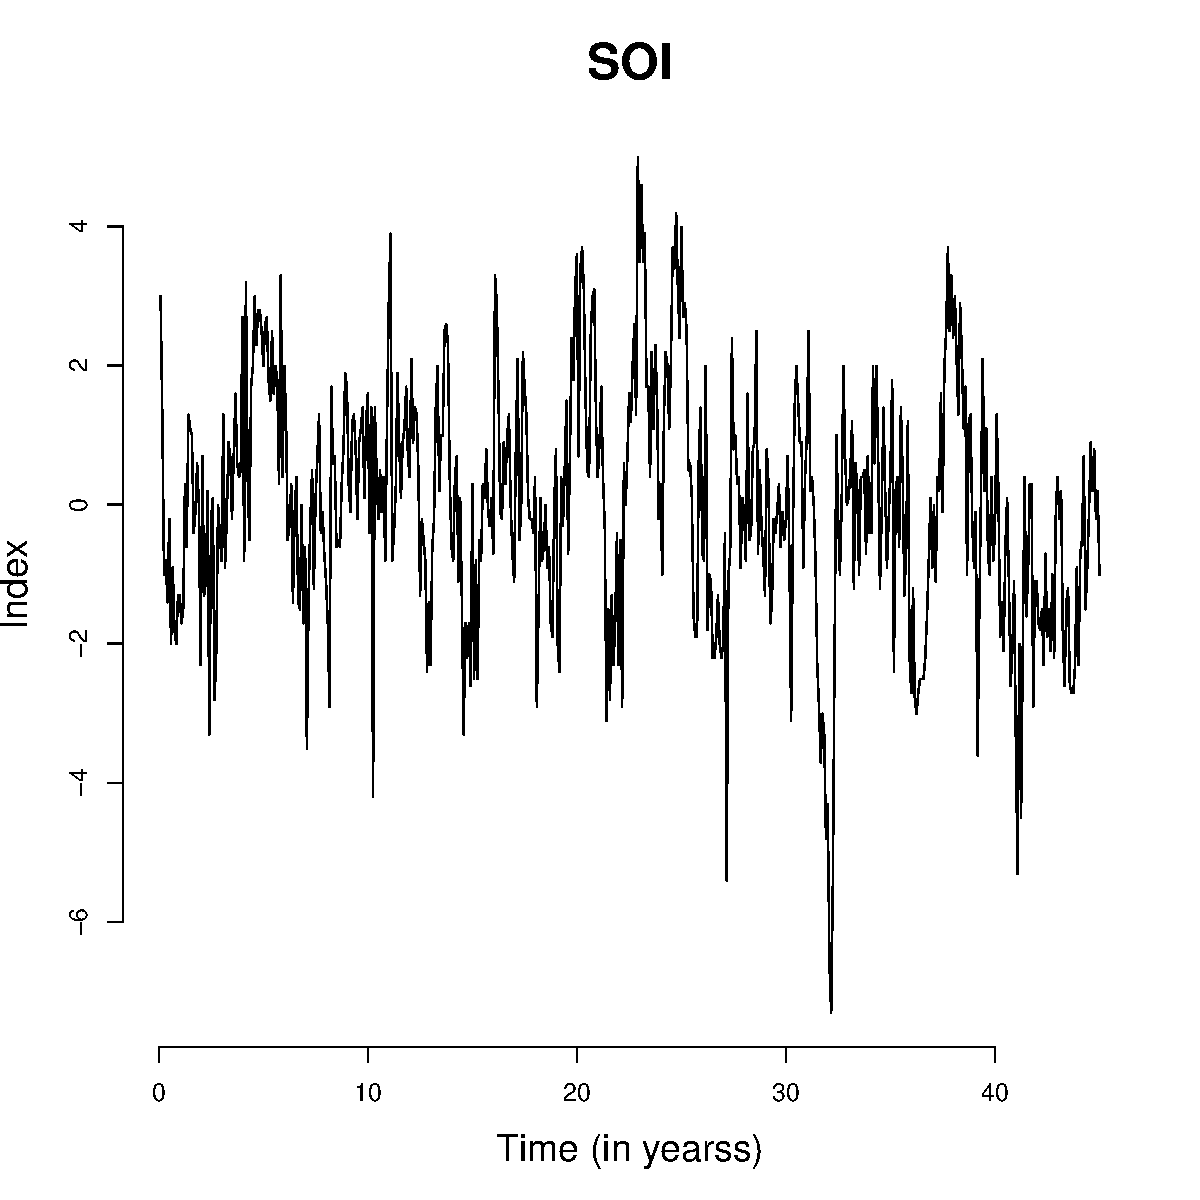
\includegraphics[scale=0.40]{dat_soi.pdf}
\end{center}
\end{figure}

\begin{figure}[H]
\begin{center}
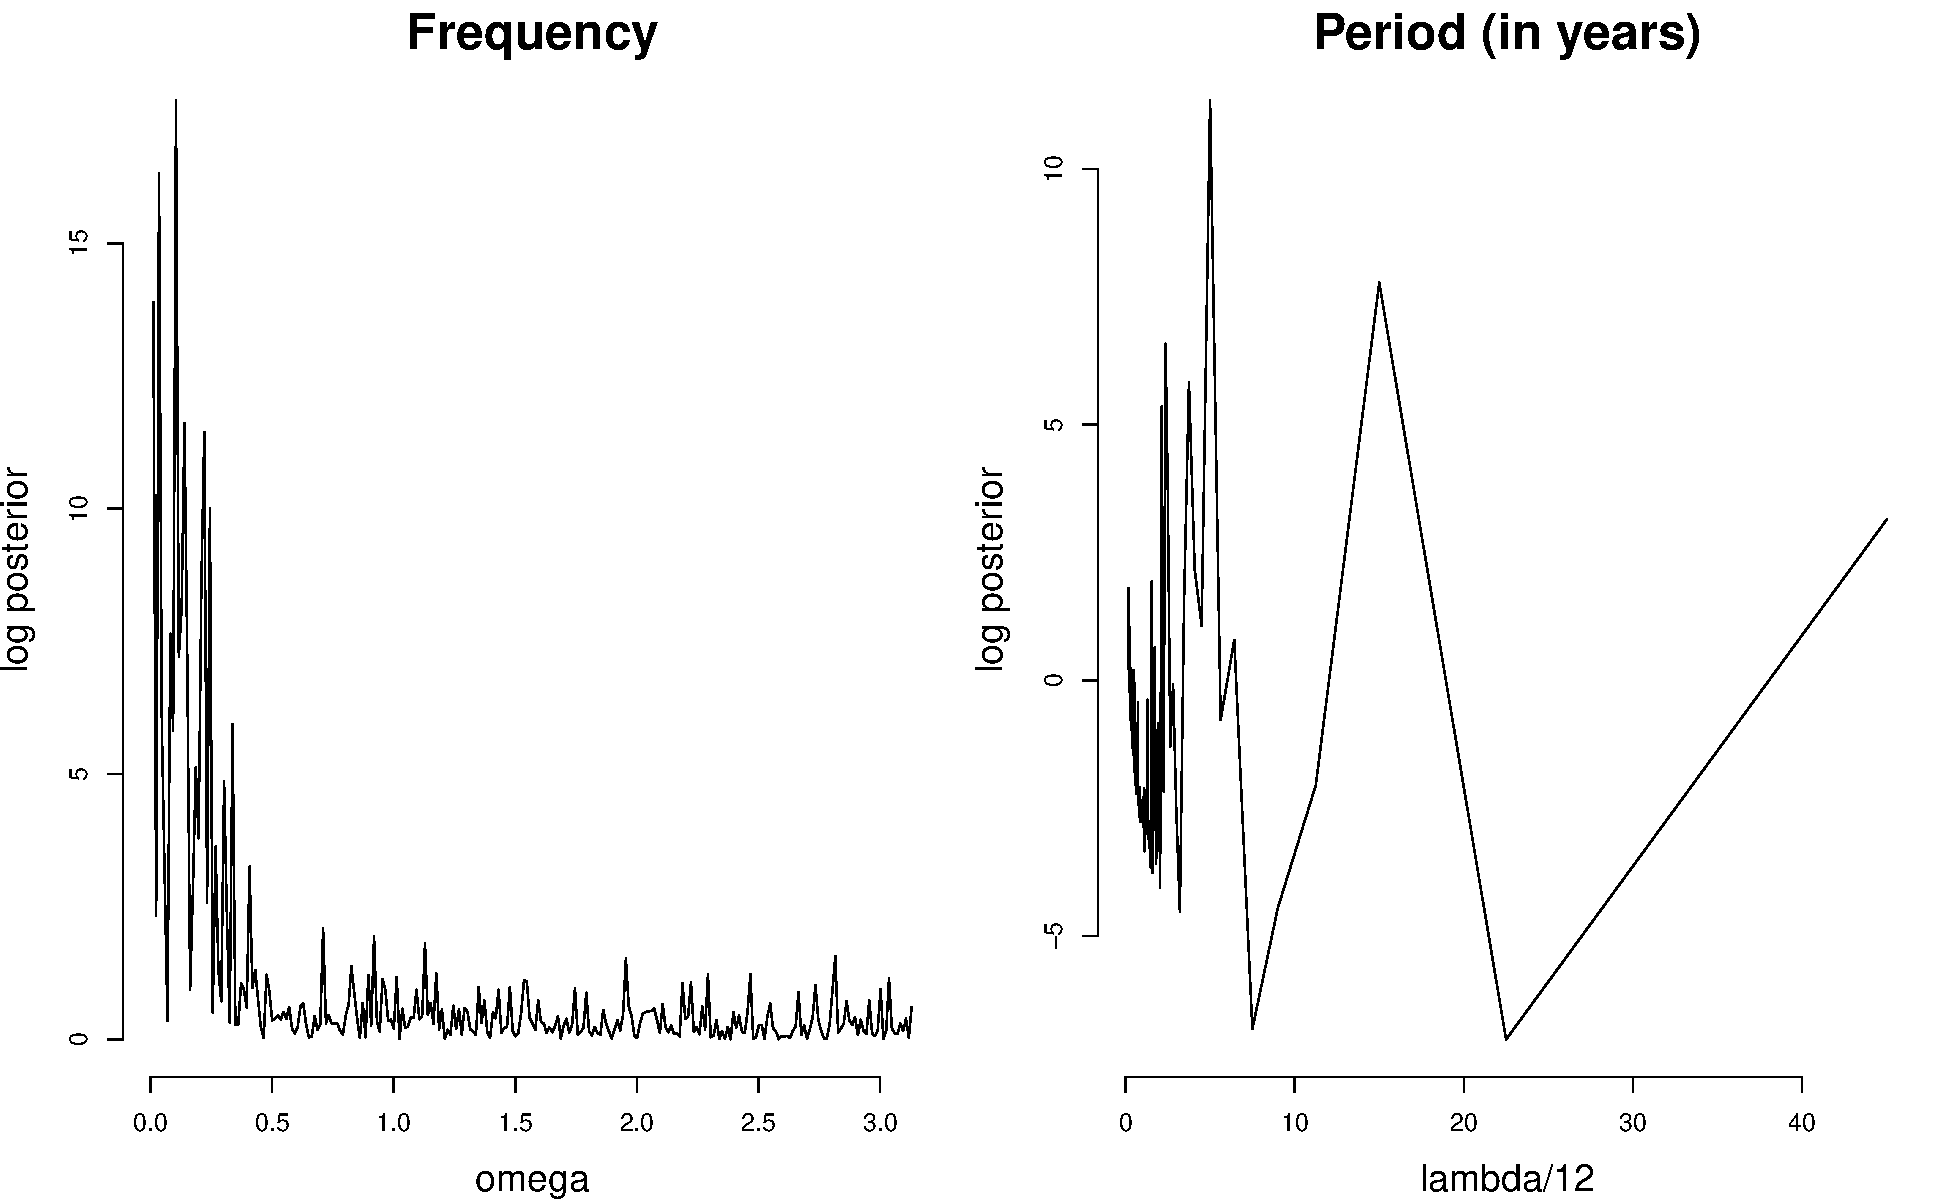
\includegraphics[scale=0.40]{fp_soi.pdf}
\end{center}
\end{figure}

\begin{figure}[H]
\begin{center}
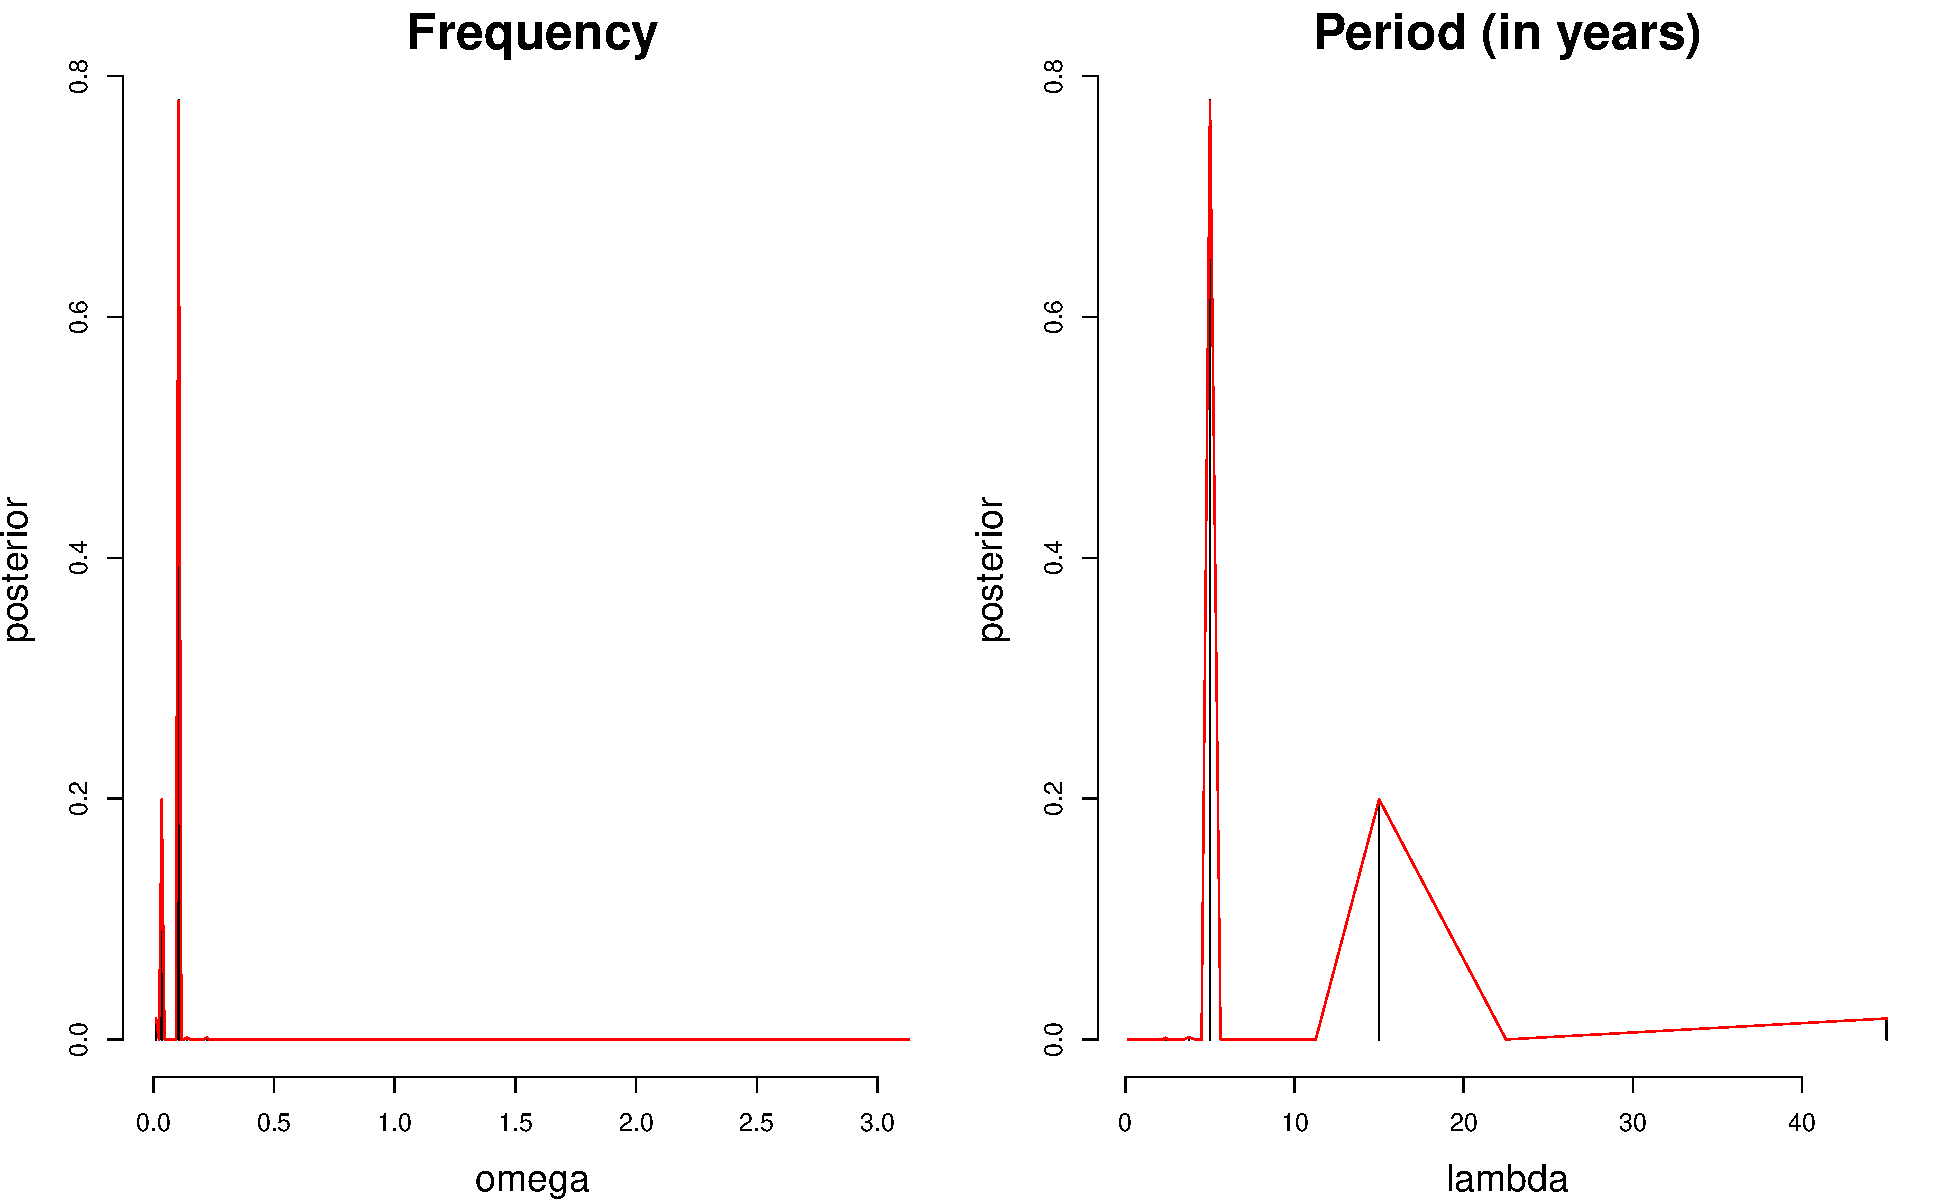
\includegraphics[scale=0.40]{sp_soi.pdf}
\end{center}
\end{figure}

\newpage

\subsection*{P\&W 3.4 -- Luteinizing hormone in blood samples}

\begin{figure}[H]
\begin{center}
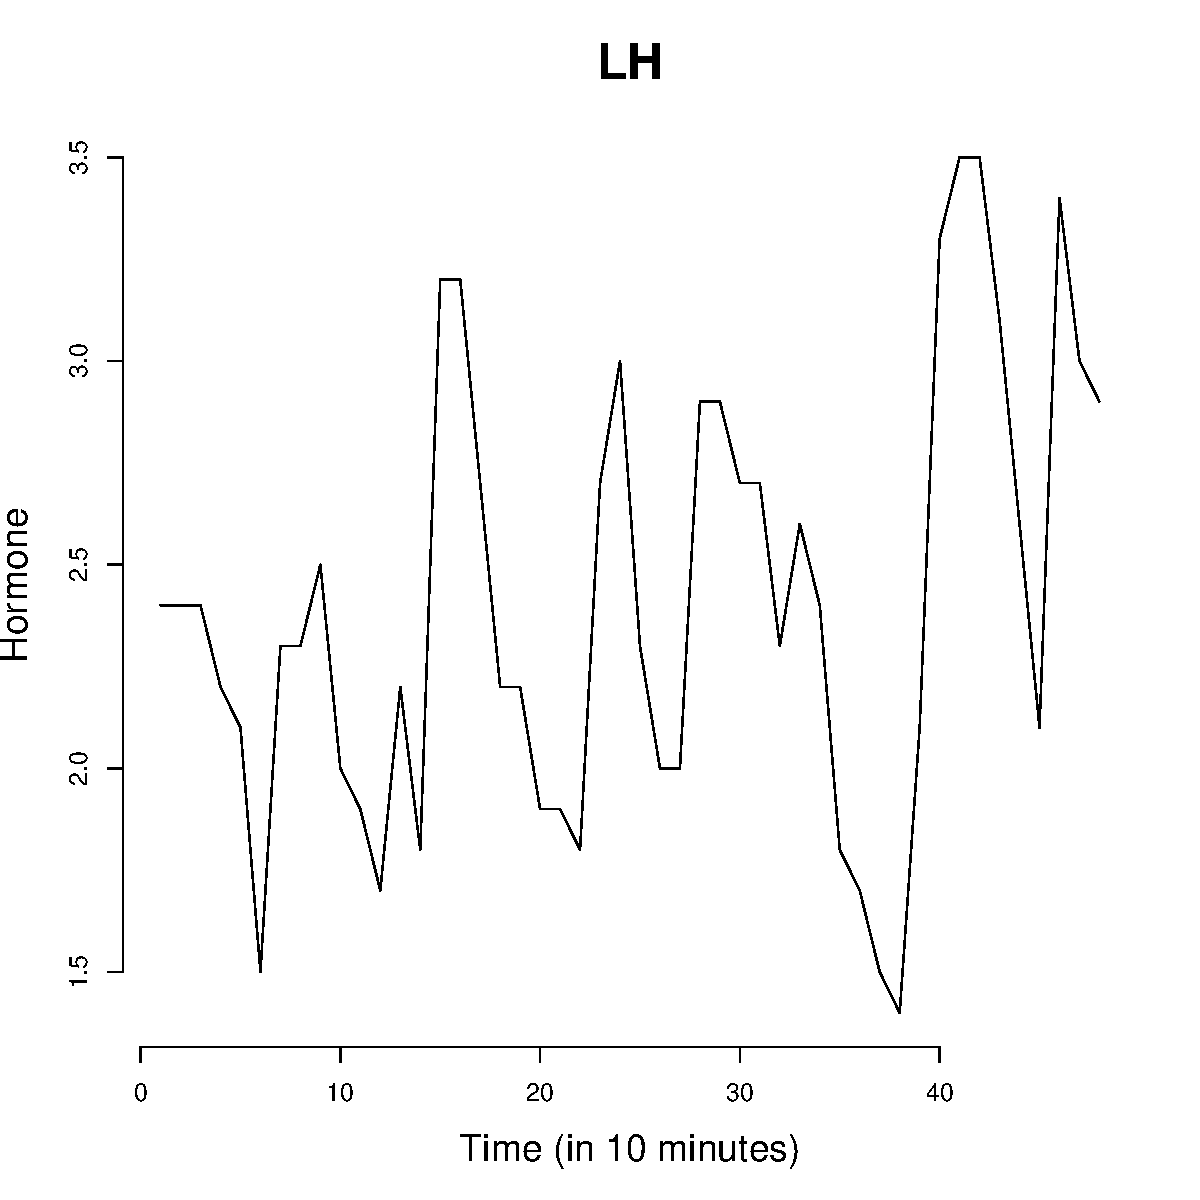
\includegraphics[scale=0.40]{dat_lh.pdf}
\end{center}
\end{figure}

\begin{figure}[H]
\begin{center}
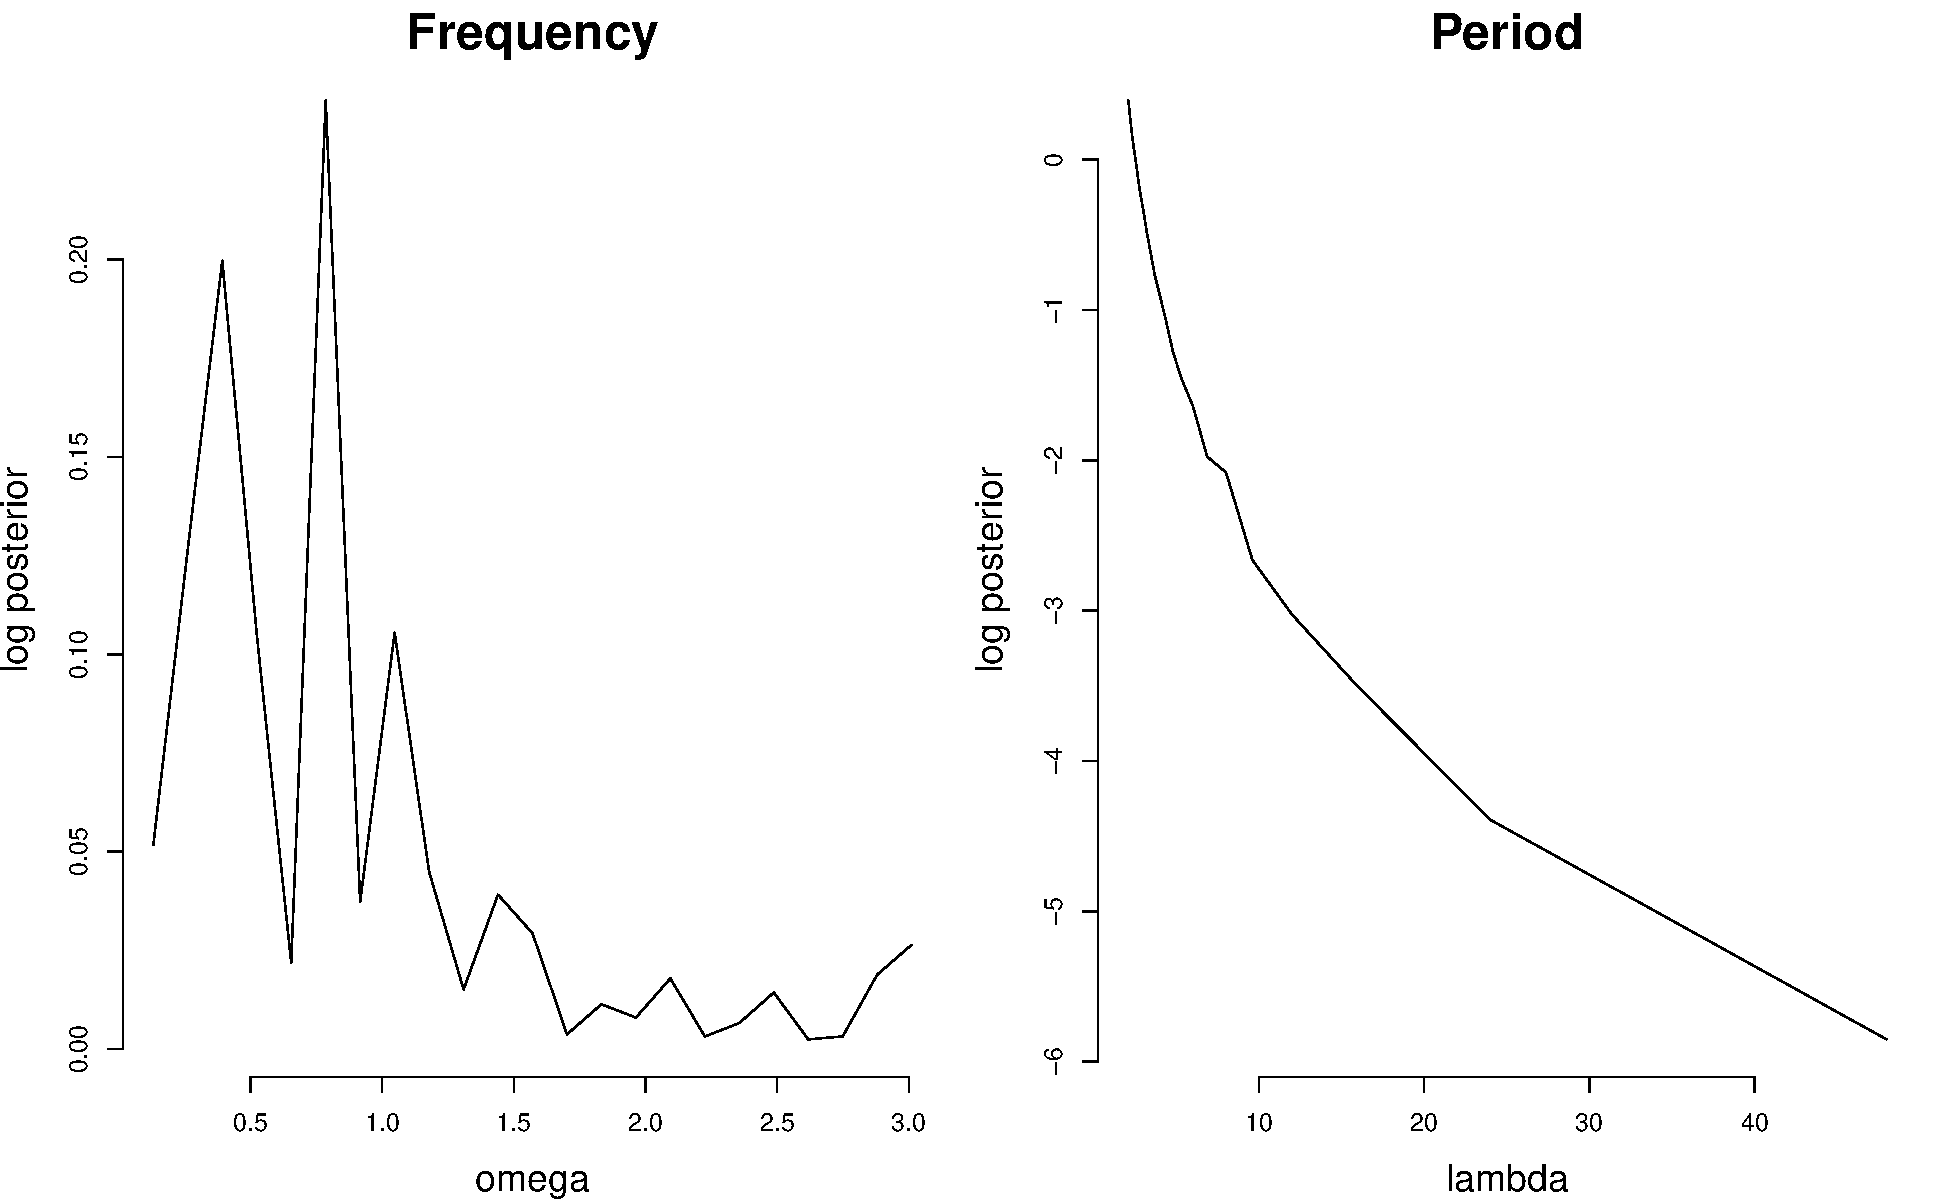
\includegraphics[scale=0.40]{fp_lh.pdf}
\end{center}
\end{figure}

\begin{figure}[H]
\begin{center}
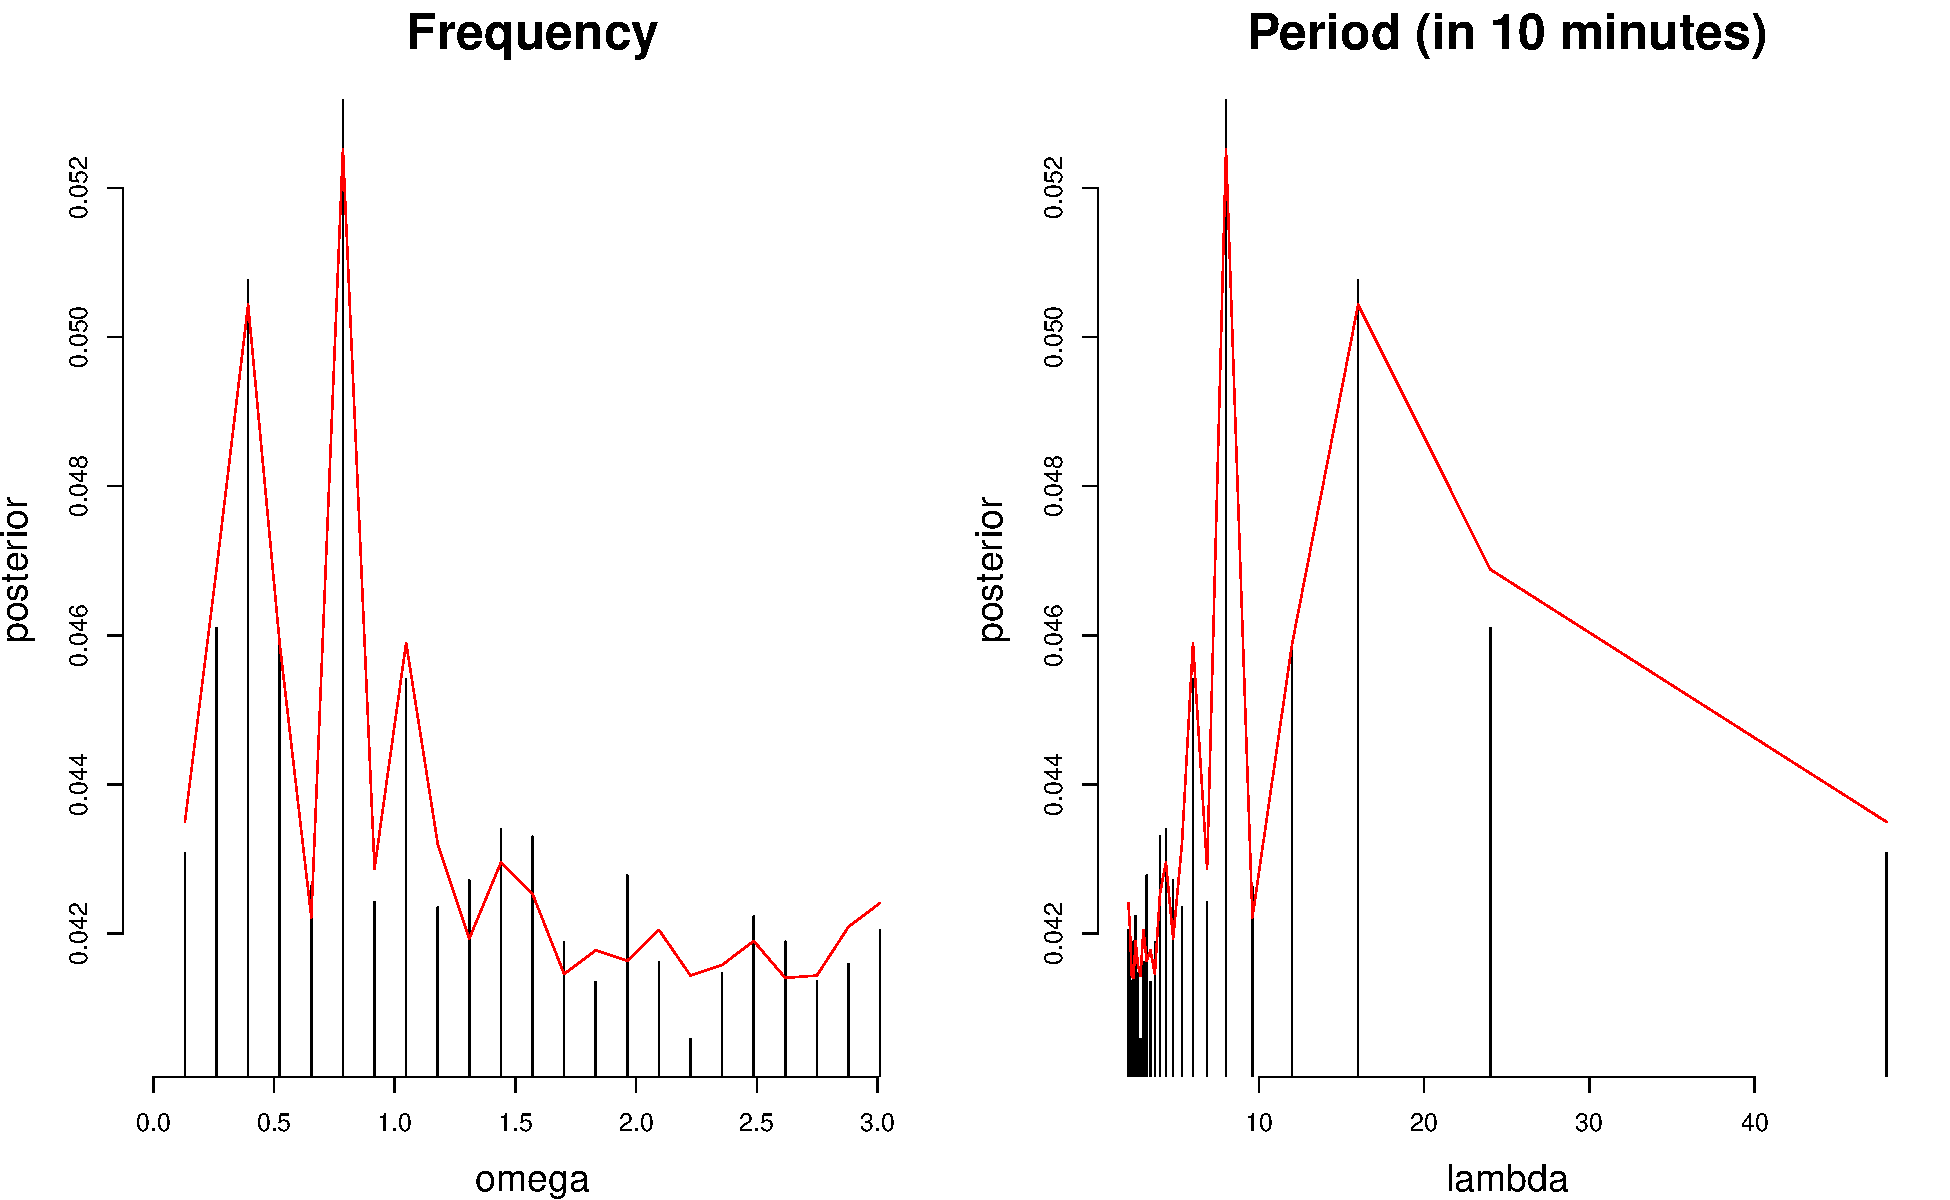
\includegraphics[scale=0.40]{sp_lh.pdf}
\end{center}
\end{figure}


\end{document}
